% Paquets généraux
\documentclass[a4paper,12pt,titlepage,twoside]{article}
\usepackage[T1]{fontenc}
\usepackage[utf8]{inputenc}
\usepackage[french]{babel}
\usepackage{subcaption}
\addto\captionsfrench{%
  \renewcommand{\tablename}{Tableau}%
}
\usepackage[gen]{eurosym}
%\usepackage[dvips]{graphicx}
\usepackage{minted}
\usepackage{fancyhdr}
\usepackage{pdfpages} 
\usepackage{multido}
\usepackage{hyperref}
\usepackage{textcomp}
\usepackage{schemabloc}
%\usepackage[bitstream-charter]{mathdesign}
\usepackage{array}
\newcolumntype{P}[1]{>{\centering\arraybackslash}p{#1}}
\usepackage[shortlabels]{enumitem}
\usepackage[framemethod=TikZ]{mdframed}

\newcommand{\id}{30}
\newcommand{\nom}{Calculs d'hyperstatisme}
\newcommand{\sequence}{04}
\newcommand{\nomsequence}{Liaisons entre les solides}
\newcommand{\num}{03}
\newcommand{\type}{TD}
\newcommand{\descrip}{En appliquant les règles de la théorie des mécanisme, déterminer le degré d'hyperstatisme de plusieurs systèmes et proposer des solutions afin de diminuer ce degré}
\newcommand{\competences}{B2-12: Proposer une modélisation des liaisons avec leurs caractéristiques géométriques. \\ &  B2-13: Proposer un modèle cinématique paramétré à partir d'un système réel, d'une maquette numérique ou d'u \\ &  B2-17: Simplifier un modèle de mécanisme. \\ &  B2-18: Modifier un modèle pour le rendre isostatique.}
\newcommand{\nbcomp}{4}
\newcommand{\systemes}{E.P.A.S, Machine d'essai de traction}
\newcommand{\systemesnum}{14, 13}
\newcommand{\systemessansaccent}{E.P.A.S, Machine d'essai de traction}
\newcommand{\ilot}{3}
\newcommand{\ilotstr}{03}
\newcommand{\dossierilot}{\detokenize{Ilot_03 E.P.A.S, Machine d'essai de traction}}
\newcommand{\imageun}{EPAS}
\newcommand{\imagedeux}{Machine_dessai_de_traction}

%\usepackage{style}
\usepackage{bodegraph}
\usepackage{rpcinematik}
\usepackage[locale = FR]{siunitx}
\usepackage{caption}
\newcommand{\institute}{Lycée Dorian}
\usepackage{calc}

\usepackage{listings}
\usepackage{fancyvrb}
\usepackage{color}
\usepackage{xcolor}
\usepackage{colortbl}
\usepackage{helvet}
\usepackage[frenchmath]{newtxsf} % for sans serif symbols
\renewcommand{\familydefault}{\sfdefault}
%\usepackage{amsfonts}
%\usepackage{amsmath}
%\usepackage{lmodern}
\usepackage{mathastext}
%\usepackage{xspace}
\usepackage{varioref}
\usepackage{tabularx}
%\usepackage{floatflt}
\usepackage{graphics}
\usepackage{wrapfig}
\usepackage{textcomp}
\usepackage{tikz,tkz-tab}
\usepackage[european resistor, european voltage, european current]{circuitikz}
\usepackage{wrapfig}
\usepackage{gensymb}
\usepackage[percent]{overpic}
\usetikzlibrary{babel}
\usepackage{ifthen}
\usepackage{cancel}
\usepackage{etoolbox}
\usepackage{multirow}
%\usepackage{boxedminipage}
\definecolor{gris25}{gray}{0.75}
\definecolor{bleu}{RGB}{18,33,98}
\definecolor{bleuf}{RGB}{42,94,171}
\definecolor{bleuc}{RGB}{231,239,247}
\definecolor{bleum}{RGB}{160,195,226}
\definecolor{rougef}{RGB}{185,18,27}
\definecolor{rougec}{RGB}{255,188,204}%255,230,231
\definecolor{vertf}{RGB}{103,126,82}
\definecolor{vertc}{RGB}{220,255,191}
\definecolor{forestgreen}{rgb}{0.13,0.54,0.13}
\definecolor{blcr}{rgb}{0.59,0.69,0.84}
\definecolor{blfr}{rgb}{0.32,0.51,0.75}
\definecolor{orfr}{rgb}{0.90,0.42,0.15}
\definecolor{orcr}{rgb}{0.90,0.65,0.50}
\definecolor{orangef}{rgb}{0.659,0.269,0.072}
\definecolor{orange}{rgb}{0.58,0.35,0.063}
\definecolor{orangec}{rgb}{0.43,0.32,0.25}
\definecolor{rcorrect}{rgb}{0.6,0,0}
\definecolor{sequence}{rgb}{0.75,0.75,0.75}
\definecolor{competences}{rgb}{0.61,0.73,0.35}
\definecolor{rose}{HTML}{ff00ff}
\definecolor{grisf}{HTML}{222222}
\definecolor{grisc}{HTML}{636363}
\definecolor{normal}{HTML}{4087c4}
\definecolor{info}{HTML}{5bc0de}
\definecolor{success}{RGB}{92,184,92}
\definecolor{warning}{RGB}{240,173,78}
\definecolor{danger}{RGB}{217,83,79}
\hypersetup{                    % parametrage des hyperliens
    colorlinks=true,                % colorise les liens
    breaklinks=true,                % permet les retours à la ligne pour les liens trop longs
    urlcolor= blfr,                 % couleur des hyperliens
    linkcolor= orange,                % couleur des liens internes aux documents (index, figures, tableaux, equations,...)
    citecolor= forestgreen                % couleur des liens vers les references bibliographiques
    }

\newcolumntype{M}[1]{>{\centering\arraybackslash}m{#1}}
\definecolor{codegreen}{rgb}{0,0.6,0}
\definecolor{codegray}{rgb}{0.5,0.5,0.5}
\definecolor{codepurple}{rgb}{0.58,0,0.82}
\definecolor{backcolour}{rgb}{0.95,0.95,0.92}

\lstdefinestyle{mystyle}{
    backgroundcolor=\color{backcolour},   
    commentstyle=\color{codegreen},
    keywordstyle=\color{magenta},
    numberstyle=\tiny\color{codegray},
    stringstyle=\color{codepurple},
    basicstyle=\ttfamily\footnotesize,
    breakatwhitespace=false,         
    breaklines=true,                 
    captionpos=b,                    
    keepspaces=true,                 
    numbers=left,                    
    numbersep=5pt,                  
    showspaces=false,                
    showstringspaces=false,
    showtabs=false,                  
    tabsize=2
}

\lstset{style=mystyle}

% Mise en page
\pagestyle{fancy}

\setlength{\hoffset}{-18pt}
\setlength{\oddsidemargin}{0pt} 	% Marge gauche sur pages impaire2s
\setlength{\evensidemargin}{0pt} 	% Marge gauche sur pages paires
\setlength{\marginparwidth}{00pt} 	% Largeur de note dans la marge
\setlength{\headwidth}{481pt} 	 	% Largeur de la zone de tête (17cm)
\setlength{\textwidth}{481pt} 	 	% Largeu\textbf{r de la zone de texte (17cm)
\setlength{\voffset}{-18pt} 		% Bon pour DOS
\setlength{\marginparsep}{7pt}	 	% Séparation de la marge
\setlength{\topmargin}{-30pt} 		% Pas de marge en haut
\setlength{\headheight}{55pt} 		% Haut de page
\setlength{\headsep}{20pt} 		% Entre le haut de page et le texte
\setlength{\footskip}{30pt} 		% Bas de\textbf{ page + séparation
\setlength{\textheight}{700pt} 		% Hauteur de l'icone zone de texte (25cm)
\setlength\fboxrule{1 pt}
\renewcommand{\baselinestretch}{1}
\setcounter{tocdepth}{1}
\newcommand{\cadre}[2]
{\fbox{
  \begin{minipage}{#1\linewidth}
   \begin{center}
    #2\\
   \end{center}
  \end{minipage}
 }
}

\newcommand{\repon}[1]
{
~\ \\
\begin{tabular}{|m{\linewidth}|}
 \hline
\multido{}{#1}{\\ \hline}
\end{tabular}
}


\newcommand{\objectif}[1]{
\mdfsetup{%
frametitle={%
\tikz[baseline=(current bounding box.east),outer sep=0pt]
\node[anchor=east,rectangle,fill=bleum]
{\strut Objectif~};}}
\mdfsetup{innertopmargin=10pt,linecolor=bleum,%
linewidth=2pt,topline=true,%
frametitleaboveskip=\dimexpr-\ht\strutbox\relax
}
\begin{mdframed}[]\relax%
#1
\end{mdframed}}


\newcounter{num_quest} \setcounter{num_quest}{0}
\newcounter{num_rep} \setcounter{num_rep}{0}
\newcounter{num_cor} \setcounter{num_cor}{0}

\newcommand{\feuilleDR}[1]{
	\begin{tikzpicture}
		\draw[gray!30](0,0)grid[step=0.5cm](\linewidth,#1);
	\end{tikzpicture}
}

%\newcommand{\question}[1]{\refstepcounter{num_quest}\par
%~\ \\ \parbox[t][][t]{0.15\linewidth}{\textbf{Question \arabic{num_quest}}}\parbox[t][][t]{0.85\linewidth}{#1\label{q\the\value{num_quest}}}\par
%}

\newcommand{\question}[1]{\refstepcounter{num_quest}\par
~\ \\ \textbf{Question \arabic{num_quest} : }#1\label{q\the\value{num_quest}}\par
}

\newcommand{\posetafigure}[3]{
\begin{figure}[ht!]
 \begin{center}
  \includegraphics[width=#2\linewidth]{img/#1}
 \end{center}
 \caption{\label{#1} #3}
\end{figure}}

\newcommand{\goforum}{
\begin{figure}

\end{figure}
\begin{center}
 \includegraphics[width=0.7\linewidth]{../../../img/go_forum}
\end{center}
\label{go_forum}
\caption{J'pète les plombs}
\end{figure}}

\newcommand{\reponse}[4][1]
{\noindent
\parbox{\textwidth}{
\rule{\linewidth}{.5pt}\\
\textbf{Question\ifthenelse{#1>1}{s}{} \multido{}{#1}{%
\refstepcounter{num_rep}\ref{q\the\value{num_rep}} }:} ~\ \\
\ifdef{\public}{#3 \ifthenelse{#2>0}{~\ \\ 	\feuilleDR{#2}}}{#4}
}}

\newboolean{printdr}
\newboolean{printcor}
\setboolean{printdr}{false}
\setboolean{printcor}{false}

\newcommand{\reponseinfo}[2][1]
{\noindent
\rule{\linewidth}{.5pt}\\
\textbf{Question\ifthenelse{#1>1}{s}{} \multido{}{#1}{%
\refstepcounter{num_rep}\ref{q\the\value{num_rep}} }:} ~\ \\
\ifdef{\public}{\parbox{\textwidth}{\ifthenelse{#2>0}{~\ \\ 	\feuilleDR{#2}}}
\setboolean{printdr}{true}\setboolean{printcor}{false}}
{\setboolean{printdr}{false}\setboolean{printcor}{true}}
}

\makeatletter
\newcommand\modulo[2]{
    \newcounter{lastpagesujet}
	\setcounter{lastpagesujet}{#1}
    \divide\value{lastpagesujet} by #2
    \multiply\value{lastpagesujet} by #2
    \advance\value{lastpagesujet} by #2
    \advance\value{lastpagesujet} by 1\relax
    }
\makeatother

\newcommand{\finsujet}[1]
{
    \begin{center}
    \Large{FIN}
    \end{center}
        
    \ifthenelse{\equal{#1}{public}}{\def\public{}}{}

	\newpage

}

\newcommand{\debutcor}
{	
    \ifdef{\public}{
    	\modulo{\value{page}-1}{4}
		\whiledo{\value{page}<\value{lastpagesujet}}{~\ \newpage}
        \pagestyle{docreponse}
	}{\pagestyle{correction}}

    \ifdef{\public}{
        \begin{tikzpicture} 
            \draw (0,0) rectangle (2,2);
            \draw (0,0) -- (2,2);
            \draw (1.5,0.5) node {\large 20};
            \draw (2.5,0) rectangle (16,2);
            \draw (4.5,1.7) node {\large Commentaires:};
        \end{tikzpicture}
    }
    ~\ \\
}

%\newcommand{\repcarre}[2]
%{
%~\ \\
%\begin{tikzpicture}
%\draw [fill=white] (0,0) rectangle +(\linewidth,#1);
%\node[align=left] at (1.1,#2-0.3) {\textbf{Question #1:}};
%\end{tikzpicture}
%}

\newcommand{\titre}[1]
{\begin{center}
\cadre{0.8}{\huge #1} 
\end{center}
}


%Définition des torseurs :
\newcommand{\torseur}[2]{\left\{\mathcal{#1}_{#2} \right\}}
\newcommand{\torseurh}[3]{\left\{\genfrac{}{}{0pt}{0}{#1}{#2}\right\}_{#3}}
\newcommand{\torseurv}[8]{\left\{
\begin{matrix}
#1 & #4 \\ #2 & #5 \\ #3 &#6
\end{matrix}
\right\}_{{#7},{#8}}}

%Définition des torseurs :
%\newcommand{\torseur}[2]{\left \{\mbox{\relsize{2}{$\mathcal {#1}$}\relsize{-2}}\phantom{}_{\mbox{\scriptsize $#2$}} \right \}}
%\newcommand{\torseurh}[3]{\left\{\genfrac{}{}{0pt}{0}{#1}{#2}\right\}_{#3}}
%\newcommand{\torseurv}[8]{
%\left\{\begin{array}{@{}c|c@{}} #1 & #4 \\ #2 & #5 \\ #3 & #6 \end{array} \right\}_{#7,#8}
%}
\newcommand{\derivee}[2]{\left.\dfrac{\d #1}{\d t}\right|_{#2}}
\newcommand{\tripleint}{\int\!\!\!\!\!\int\!\!\!\!\!\int}

% Notation cinématique et statique
\newcommand{\cinematique}[2]{\mbox{#1}/\mbox{#2}}
\newcommand{\statique}[2]{\mbox{#1}\rightarrow\mbox{#2}}
\newcommand{\moment}[3]{\vv {#1}_{\scriptsize{#3}}(#2)}
\newcommand{\resultante}[2]{\vv {#1}_{\scriptsize{#2}}}


%Commande de base
\newcommand{\jo}{\left(j\omega\right)} % j \omega dans l'analyse fréquentielle
\newcommand{\tl}{\xrightarrow{\mathcal{L}}} % transformée de laplace sur fleche
\newcommand{\tli}{\xrightarrow{\mathcal{L}^{-1}}} % transformée inverse de laplace sur fleche
\renewcommand{\d}[1][]{\mathrm{d#1}}
\newcommand{\dd}[1][]{\mathrm{d#1}}
\newcommand{\vect}[2]{{#1}\wedge{#2}}
\newcommand{\base}[3]{(\vec #1,\vec #2,\vec #3)}
\newcommand{\vectbase}[4]{{\vphantom{\left| \begin{matrix}
#1\\#2\\#3 \end{matrix} \right|}}_{#4}{\left| \begin{matrix}
#1\\#2\\#3 \end{matrix} \right.}}
%Pour avoir les paragraphes sous la forme I, II, III
\renewcommand{\thesection}{\Roman{section}}
\setcounter{secnumdepth}{3}
\renewcommand{\Frlabelitemii}{$\bullet$}

% En tête et pied de page
\lhead{\nom}
\rhead{\includegraphics[width=2cm]{../../../img/logo}}
\lfoot{\auteurun,\ \auteurdeux}
\cfoot{Page \thepage}

\fancypagestyle{docreponse}{%
  \fancyhf{}
  \fancyhead[LO]{NOM Prénom: .............................}
  \rhead{\includegraphics[width=2cm]{../../../img/logo}\hspace{2pt}}
  \ifdef{\auteurdeux}{\lfoot{\auteurun,\ \auteurdeux}}{\lfoot{\auteurun}}
  \rfoot{\nom}
  \lfoot{Document réponse}
  \cfoot{Page \thepage}
   }

\fancypagestyle{correction}{%
  \fancyhf{}
  \lhead{\colorbox{danger}{\begin{minipage}{0.65\paperwidth} \textcolor{white}{\textbf{Correction}} \end{minipage}} }
  \rhead{\includegraphics[width=2cm]{../../../img/logo}}
  \lfoot{Renaud Costadoat, Françoise Puig}
  \rfoot{\colorbox{danger}{\begin{minipage}{0.3\paperwidth} \begin{flushright}\textcolor{white}{\textbf{Correction}}\end{flushright} \end{minipage}} }
  \cfoot{Page \thepage}
}

\fancypagestyle{correctioninfo}{%
  \fancyhf{}
  \lhead{\colorbox{danger}{\begin{minipage}{0.65\paperwidth} \textcolor{white}{\textbf{Correction}} \end{minipage}} }
  \rhead{\includegraphics[width=2cm]{../../../img/logo}}
  \lfoot{Renaud Costadoat, Juliette Genzmer}
  \rfoot{\colorbox{danger}{\begin{minipage}{0.6\paperwidth} \begin{flushright}\textcolor{white}{\textbf{Correction}}\end{flushright} \end{minipage}} }}

\renewcommand{\footrulewidth}{0.4pt}

\usepackage{eso-pic}
\newcommand{\BackgroundPic}{%
\put(0,0){%
\parbox[b][\paperheight]{\paperwidth}{%
\vfill
\begin{center}
\hspace{0.5cm}\vspace{0.5cm}
\includegraphics[width=\paperwidth,height=\paperheight,%
keepaspectratio]{../../../img/fond3}%
\end{center}
\vfill
}}}

\newcommand{\BackgroundPicdeux}{%
\put(25,-30){%
\parbox[b][\paperheight]{\paperwidth}{%
\vfill
\begin{center}
\includegraphics[width=\paperwidth,height=\paperheight,%
keepaspectratio]{../../../img/fond4}%
\end{center}
\vfill
}}}

\begin{document}

\pagestyle{empty}

\AddToShipoutPicture*{\BackgroundPic}

\includegraphics[width=2cm]{../../../img/logo}

\Huge{DS \numero - \sujet}

\vspace{1cm}

\ifdef{\prive}{\begin{center}\colorbox{danger}{\Huge{Avec Correction}}\end{center}}{}

\begin{center}
\centering\huge{PTSI}
\end{center}

\vspace{2cm}


\begin{center}
\centering\Large{\jour}
\end{center}

\vspace{2cm}

\normalsize

\tableofcontents

\newpage

\AddToShipoutPicture{\BackgroundPicdeux}

\pagestyle{fancy}

\begin{center}
\Huge \sujet
\end{center}


\normalsize


\section{Introduction}

\begin{figure}[ht!]
\begin{center}
\includegraphics[width=.6\linewidth]{img/fig00}
\caption{\label{fig00}Vélo cargo}
\end{center}
\end{figure}

\vspace{-1cm}

Le secteur des transports est la première source d'émissions de gaz à effet de serre en France avec 31\% des
émissions du pays. Ces émissions sont, pour plus de moitié, dues aux véhicules individuels motorisés (voitures,
motos) qui restent utilisés au quotidien par 68\% des Français alors que plus de la moitié des trajets effectués fait moins de 5 km\footnote{Données extraites de l'article « Bouger autrement au quotidien » publié par l'ADEME https://librairie.ademe.fr/cadic/7338/guide-bouger-autrement-au-quotidien.pdf}.

À l'inverse, non content d'être un très faible émetteur de gaz à effet de serre, le vélo s'avère peu consommateur en ressources et en énergie tout en étant bon pour la santé individuelle et collective. Le vélo constitue également une solution viable pour décongestionner les villes. Son utilisation est encouragée par de nombreux acteurs institutionnels de par la création d'aménagements cyclables, les aides à l'achat de vélo à assistance électrique ou encore la création du forfait mobilité durable.

L'essor des vélos à assistance électrique (VAE) a libéré de nombreux cyclistes de l'appréhension du relief. Le
développement des VAE s'est accompagné de celui des vélos cargos qui permettent d'effectuer des livraisons ou
encore de transporter des enfants. Ce sujet porte sur un de ces vélos cargo.

\subsection{Présentation du système}

La société Douze cycles conçoit et réalise des vélos cargo destinés aux professionnels comme aux particuliers.
Cette société est implantée en Bourgogne où elle emploie 25 collaborateurs.

Le système étudié est un biporteur à assistance électrique, le G4e, conçu et réalisé par Douze cycles. Soucieuse d'allier durabilité, praticité et esthétique, la société Douze cycles innove continument pour faire évoluer sa gamme de produits. Ce vélo, présenté par l'entreprise comme « une solution vélogistique tout-en-un répondant à la plupart des usages pour les familles ou les professionnels », a été lancé en 2017 pour le cinquième anniversaire de la marque.

\subsection{Étude proposée}

Les études proposées dans ce sujet portent sur différentes problématiques spécifiques à la conception du vélo
cargo étudié :
\begin{itemize}
 \item L'étude s'ouvre, partie 2 sur la détermination de l'effort que doit fournir le cycliste pour garer le vélo sur sa béquille,
 \item La modélisation du capteur utilisé pour mesurer le couple appliqué par le cycliste sur le pédalier occupe la partie 3,
 \item La partie 4 se focalise sur l'étude de l'association \{ onduleur + machine \} qui anime le groupe d'assistance,
 \item Enfin, les modèles obtenus lors des deux parties précédentes sont exploités partie 5 lors de l'étude de
l'asservissement du couple délivré par la machine.
\end{itemize}

\section{Effort de mise en stationnement}

\paragraph{Objectif} Déterminer l'effort à exercer par l'usager lors de la mise en stationnement sur béquille.

~\

La mise en position parking du vélo cargo (le « béquillage ») nécessite d'exercer un effort sur le guidon. Cette partie vise à déterminer cet effort et à vérifier sa compatibilité avec les exigences d'ergonomie.

\begin{figure}[ht!]
\begin{center}
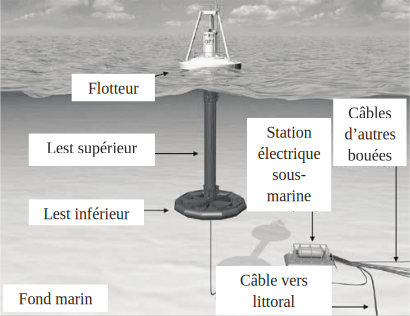
\includegraphics[width=.95\linewidth]{img/fig01}
\caption{\label{fig01}Extrait du cahier des charges relatif à l'ergonomie de la mise en stationnement du vélo}
\end{center}
\end{figure}

\newpage

\begin{figure}[ht!]
\begin{minipage}{0.7\linewidth}
\begin{center}
\includegraphics[width=\linewidth]{img/fig02}
\caption{\label{fig02}Paramétrage adopté pour la détermination des caractéristiques inertielles du vélo}
\end{center}
\end{minipage}\hfill
\begin{minipage}{0.27\linewidth}
\begin{itemize}
 \item $\overrightarrow{IJ}=L\cdot \vec{x}$
 \item $L=2050mm$
 \item $\overrightarrow{IG_v}=x_G\cdot \vec{x}+y_G\cdot \vec{y}$
 \item $\overrightarrow{IG_B}=x_B\cdot \vec{x}+y_B\cdot \vec{y}$
 \item $x_B=1250mm$
 \item $\overrightarrow{IG_T}=x_T\cdot \vec{x}+y_T\cdot \vec{y}$
\end{itemize}
\end{minipage}
\end{figure}

\subsection{Caractéristiques inertielles du vélo}

\paragraph{Définition des ensembles}
\begin{itemize}
 \item $V$ : ensemble du vélo hors béquille (supposée de masse négligeable) et hors black-box,
 \item $B$ : black-box chargée au maximum,
 \item $T =V \cup B$.
\end{itemize}

\subsubsection{Centre de gravité $G_V$ du vélo à vide}

On étudie le vélo G4e à vide (ensemble $V$). La masse totale de cet ensemble est alors $m_V = 50 kg$. Les roues du vélo ainsi équipé sont positionnées sur des balances, l'ensemble étant en équilibre dans le plan vertical $(I,\vec{x},\vec{y})$. On mesure au niveau des points de contact :
\begin{itemize}
 \item arrière, I : $m_I = 26 kg$,
 \item avant, J : $m_J = 24 kg$.
\end{itemize}

La distance entre les points I et J est notée $L = 2050 mm$ (voir figure \ref{fig02}).

\question{Déterminer l'expression littérale de la position $x_G$ suivant $\vec{x}$ du centre de gravité de l'ensemble. En déduire la valeur de $x_G$ en mm.}

\subsubsection{Centre de gravité GT du vélo chargé}

On considère à présent que la black box est chargée à son maximum ($m_B = 100 kg$). On appelle $G_B$, le centre de gravité de la masse chargée où $x_B = 1250 mm$.

\question{Déterminer l'expression littérale de la position $x_T$ suivant $\vec{x}$ du centre de gravité de l'ensemble chargé. Calculer la valeur de $x_T$.}

\subsection{Étude géométrique}

L'étude est menée dans le plan $(I,\vec{x},\vec{y})$ à partir du paramétrage défini figure \ref{fig03}.

\paragraph{Procédure de béquillage} Le béquillage se réalise en poussant la béquille avec le pied sur le sol puis en exerçant une action de traction sur le guidon.

L'utilisateur garde son pied sur la béquille pour la plaquer au sol durant toute la phase de béquillage afin de maintenir le contact en K de la béquille avec le sol.

\paragraph{Mouvement du vélo} On suppose dans cette partie que la fourche avant est rigide durant la phase de béquillage. Dès lors, la roue avant se décollera du sol sous l'action de traction du vélo par l'usager tandis que la roue arrière reculera.

\paragraph{Définition de l'ensemble étudié :} L'ensemble étudié se compose des solides suivants :
\begin{itemize}
 \item le sol (0), repère associé $(I,\vec{x},\vec{y},\vec{z})$,
 \item la roue arrière (1),
 \item le cadre (2), repère associé $(A,\vec{x_c},\vec{y_c},\vec{z})$,
 \item la béquille (4), repère associé $(A,\vec{x_b},\vec{y_b},\vec{z})$,
 \item la roue avant (3).
\end{itemize}

\paragraph{Modèle cinématique} On modélise la cinématique de l'ensemble par une liaison :
\begin{itemize}
 \item sphère/plan de normale $(I,\vec{y})$ entre la roue arrière (1) et le sol (0),
 \item pivot d'axe $(B,\vec{z})$ entre la roue (1) et le cadre (2),
 \item pivot d'axe $(A,\vec{z})$ entre le cadre (2) et la béquille (4),
 \item pivot d'axe $(K,\vec{z})$ entre la béquille (4) et le sol (0) (modélisation associée au blocage de la béquille par le pied).
\end{itemize}

\begin{figure}[ht!]
\begin{center}
\includegraphics[width=0.8\linewidth]{img/fig03}
\caption{\label{fig03}Paramétrage utilisé pour l'étude du béquillage}
\end{center}
\end{figure}

\begin{minipage}{0.3\linewidth}
\begin{itemize}
 \item $\overrightarrow{KI}=\mu(t)\cdot \vec{x}$
 \item $\overrightarrow{KA}=a\cdot \vec{x_b}$
 \item $\overrightarrow{IB}=R_B\cdot \vec{y}$
 \item $\overrightarrow{AB}=-b\cdot \vec{x_c}+e\cdot \vec{y_c}$
 \item $\overrightarrow{AG_T}=(x_T-b)\cdot \vec{x_c}+(y_T-h)\cdot \vec{y_c}$
 \end{itemize}
\end{minipage}\hfill
\begin{minipage}{0.3\linewidth}
\begin{itemize}
 \item $a=290mm$
 \item $R_B=340mm$
 \item $b=1030mm$
 \item $e=70mm$
 \item $h=270mm$
 \item $x_T=1150mm$
 \item $y_T=400mm$
\end{itemize}
\end{minipage}\hfill
\begin{minipage}{0.35\linewidth}
\begin{itemize}
 \item $\alpha(t)=(\vec{x},\vec{x_b})=(\vec{y},\vec{y_b})$
 \item $\beta(t)=(\vec{x},\vec{x_c})=(\vec{y},\vec{y_c})$
\end{itemize}
La partie basse du cadre est à l'horizontale avant le béquillage :
$\vec{x_c}$ et $\vec{x}$ sont colinéaires lorsque les deux roues sont en contact
avec le sol.
\end{minipage}

\question{Compléter le schéma cinématique esquissé sur le document réponse conformément au
modèle proposé en faisant apparaître les liaisons, les solides et les repères qui leurs sont associés.}

\question{Compléter les figures de changement de base esquissées sur le document réponse.}

\question{À partir d'une fermeture géométrique, montrer que l'équation scalaire qui lie la valeur de $\beta$ à $\alpha$, $a$, $b$, $e$ et $R_B$ est de la forme : $a\cdot sin(\alpha) = b \cdot sin(\beta) - e \cdot cos(\beta) + R_B$.}

\paragraph{Valeurs limites de $\alpha$} On note $\alpha_i$ et $\alpha_f$ ($\alpha_i < \alpha_f$ ) les valeurs de l'angle $\alpha$ entre lesquelles la roue avant est décollée du sol. On suppose que $\beta$ étant faible, $cos\beta=1$ et $sin\beta=0$.

\question{Déterminer les expressions des angles $\alpha_i$ et $\alpha_f$ en fonction de $R_B$, $e$ et $a$. En calculer les valeurs en degrés.}

\begin{figure}[!ht]
\begin{minipage}{0.55\linewidth}
\begin{center}
\includegraphics[width=0.9\linewidth]{img/fig04a}
\caption{\label{fig04a}Tracé de $sin\theta$ en fonction de $\theta$.}
\end{center}
\end{minipage}
\begin{minipage}{0.5\linewidth}
\begin{center}
\includegraphics[width=0.7\linewidth]{img/fig04b}
\caption{\label{fig04b}Évolution de $\beta$ en fonction de $\alpha$ au cours du béquillage.}
\end{center}
\end{minipage}
\end{figure}

Les valeurs calculées précédemment arrondies conduisent à $\alpha_i\approx 70\degree$ et $\alpha_f\approx 110\degree$. L'évolution de l'angle $\beta$ en fonction de $\alpha$, pour la plage de béquillage, est donnée figure \ref{fig04b} ci-contre.

\question{Déduire de la courbe fournie la valeur d'inclinaison maximale du cadre par rapport au sol, notée $\beta_{max}$. Conclure sur l'hypothèse d'étude suivante : \og Le cadre sera supposé horizontal lors du béquillage \fg.}


\subsection{Effort de béquillage}

On se propose à présent d'estimer l'action mécanique que doit développer le cycliste sur le guidon lors du
béquillage dans le cas où la béquille est perpendiculaire au cadre ($\alpha = 90\degree$, on admet qu'il s'agit de la position critique en termes d'effort). Le paramétrage adopté pour cette étude est défini figure \ref{fig05}.

\begin{figure}[!ht]
\begin{center}
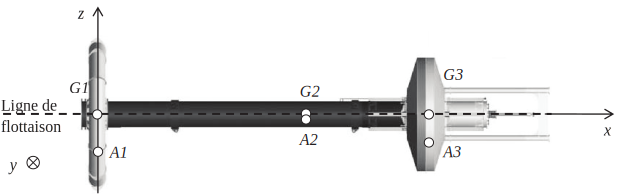
\includegraphics[width=0.8\linewidth]{img/fig05}
\caption{\label{fig05}Paramétrage utilisé pour l'étude du béquillage}
\end{center}
\end{figure}

\begin{minipage}{0.3\linewidth}
\begin{itemize}
 \item $\overrightarrow{KI}=\mu(t)\cdot \vec{x}$
 \item $\overrightarrow{KA}=a\cdot \vec{y}$
 \item $\overrightarrow{KG_T}=k\cdot \vec{x_c}+q\cdot \vec{y_c}$
 \item $\overrightarrow{AM}=-d\cdot \vec{x_c}+y_M\cdot \vec{y_c}$
 \end{itemize}
\end{minipage}\hfill
\begin{minipage}{0.3\linewidth}
\begin{itemize}
 \item $a=290mm$
 \item $\mu=-1030mm$
 \item $k=120mm$
 \item $q=130mm$
 \item $d=180mm$
 \item $y_M\in [900,1000]mm$
\end{itemize}
\end{minipage}\hfill
\begin{minipage}{0.36\linewidth}
\begin{itemize}
 \item $\alpha(t)=(\vec{x},\vec{x_B})=(\vec{y},\vec{y_B})=90\degree$
 \item $\beta(t)=(\vec{x},\vec{x_C})=(\vec{y},\vec{y_C})=1\degree$
\end{itemize}
\end{minipage}

\paragraph{Notation} Le torseur de l'action mécanique exercée par le solide i sur j, dans la base $(\vec{x},\vec{y},\vec{z})$, dans l'hypothèse de problème plan, est noté :

$$\left\{T_{i\rightarrow j}\right\}=\left\{
\begin{array}{cc}X_{ij}&\sim\\Y_{ij}&\sim\\ \sim&N_{ij}^K
\end{array}\right\}_{K,(\vec{x},\vec{y},\vec{z})}\ ou\ \left\{T_{i\rightarrow j}\right\}=\left\{
\begin{array}{c}X_{ij}\cdot\vec{x}+Y_{ij}\cdot\vec{y}\\N_{ij}^K\cdot\vec{z}
\end{array}\right\}_K$$

Données et hypothèses
\begin{itemize}
 \item L'action mécanique exercée par le cycliste est un glisseur $\overrightarrow{F_C}$ appliqué en M tel que $\overrightarrow{F_C}=-F_C\cdot \vec{x}$,
 \item L'accélération de la pesanteur vaut $\vec{g} = -g\cdot\vec{y}$ où on approche $g$ par $g = 10 m\cdot s^{-2}$,
 \item La masse de l'ensemble, pour rappel, est notée $m_T$ et vaut $m_T = 150 kg$,
 \item On suppose les liaisons sans frottements à l'exception du contact Roue/Sol, où l'on suppose un frottement suivant le modèle de Coulomb de coefficient $f = 1$.
\end{itemize}

\question{Donner la forme du torseur des actions mécaniques transmissibles du sol (0) sur la béquille (4) en K dans la base $(\vec{x},\vec{y},\vec{z})$.}

\question{Donner la forme du torseur des actions mécaniques transmissibles du sol (0) sur la roue (1) en I dans la base $(\vec{x},\vec{y},\vec{z})$.}

\question{Donner la forme du torseur des actions mécaniques exercées par la pesanteur sur l'ensemble $\sum=\{1, 2, 3, 4\}$ en $G_T$ dans la base $(\vec{x},\vec{y},\vec{z})$.}

\question{Appliquer le théorème du moment statique à $\sum$ en I en projection sur $\vec{z}$. En déduire la
relation qui lie $F_C$ à $Y_{04}$ en fonction de $\mu$, $a$, $k$, $q$, $d$, $y_M$ , $\beta$, $m_T$ et $g$.}

~\

On rappelle que $\beta$ est suffisamment petit pour considérer que $sin \beta \approx 0$ et $cos \beta \approx 1$.

\question{Montrer qu'alors, on peut exprimer $F_C$ sous la forme :
$$F_C\approx\dfrac{\mu\cdot Y_{04}-(\mu-k)\cdot m_T\cdot g}{y_M+a}$$

Déterminer la condition sur $y_M$ qui conduit alors à une action à développer par le cycliste $F_C$ maximale.}

\question{En isolant l'ensemble $\sum$ et en appliquant le théorème de la résultante statique, écrire les
équations scalaires qui relient les différentes composantes des torseurs d'actions mécaniques exercées par le sol.}

\question{Montrer alors, que même en supposant le glissement en I, l'isolement de l'ensemble ne
permet pas de déterminer l'action du cycliste.}

~\

On se propose à présent d'isoler la béquille (4) seule. On fait l'hypothèse que son poids est négligeable devant les autres actions mécaniques.

\question{Montrer en appliquant le PFS à la béquille (4) et en choisissant une équation scalaire pertinente parmi celles disponibles, que pour la position étudiée ($\alpha=90\degree$) et pour l'isolement choisi, $X_{04}=0$.}

~\

On montre alors en utilisant les résultats précédents :

$$F_C=\dfrac{f\cdot k\cdot m_T\cdot g}{\mu+f\cdot (y_M+a)}$$

On estime alors l'effort minimal pour assurer le béquillage en charge maximale à $F_C\approx 80 N$.

\question{Conclure sur le respect de l'exigence 110 du cahier des charges du vélo (figure \ref{fig01})}

\section{Étude du capteur de couple}

Le groupe d'assistance dont est pourvu le vélo cargo assiste le cycliste en fonction du couple que celui-ci
applique sur le pédalier. Ce groupe d'assistance comporte donc un capteur destiné à acquérir le couple appliqué
par le cycliste sur le pédalier. Cette section vise à modéliser ce capteur et à en dimensionner certains éléments.

\begin{figure}[ht!]
\begin{center}
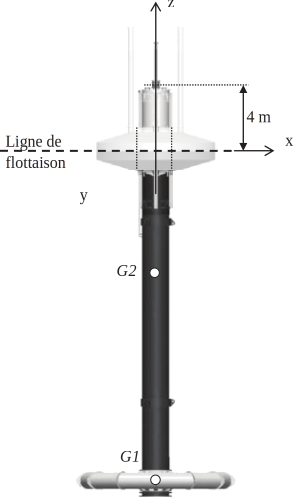
\includegraphics[width=.8\linewidth]{img/fig06}
\caption{\label{fig06}Extrait du cahier des charges relatif à la mesure du couple appliqué par l'utilisateur sur le pédalier.}
\end{center}
\end{figure}

\subsection{Présentation du capteur}

Le capteur utilisé est composé d'un transducteur à reluctance variable (présenté ci-dessous), d'un circuit
d'amplification et de détection d'amplitude (non étudié) et d'un convertisseur analogique numérique.

\begin{figure}[ht!]
\begin{center}
\includegraphics[width=.8\linewidth]{img/fig07}
\caption{\label{fig07}Extrait du cahier des charges relatif à la mesure du couple appliqué par l'utilisateur sur le pédalier.}
\end{center}
\end{figure}

\paragraph{Constitution du transducteur à reluctance variable} Un schéma de principe du transducteur à reluctance variable autour duquel est construit le capteur de couple étudié est donné figure \ref{fig08}. Ce transducteur est constitué de quatre ensembles :
\begin{itemize}
 \item l'arbre A1 sur lequel est monté un anneau magnétique Am1,
 \item l'arbre A2 sur lequel sont montés les anneaux magnétiques Am21 et Am22,
 \item l'arbre de torsion At qui relie les arbres A1 et A2,
 \item un bâti (non représenté sur la figure \ref{fig08}). Les arbres A1 et A2 sont guidés en rotation par rapport à ce bâti. Les bobines de détection Bd et de compensation Bc sont solidaires du bâti.
\end{itemize}

\paragraph{Principe de la mesure} Les bobines Bd et Bc sont alimentées par une source de tension sinusoïdale.
Le circuit magnétique constitué par la bobine de compensation et les anneaux magnétiques Am21 et Am22
est indéformable. Son inductance est donc indépendante du couple transmis (cette bobine sert à compenser la
dérive en température).

Le circuit magnétique constitué par la bobine de détection et les anneaux magnétiques Am1 et Am21 se
déforme en même temps que l'arbre de torsion. Cette déformation provoque une variation de l'inductance de la
bobine de détection. Le transducteur est construit de telle sorte que cette variation d'inductance soit proportionnelle au couple à mesurer.

\begin{figure}[ht!]
\begin{center}
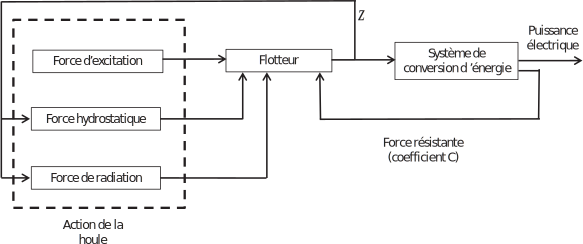
\includegraphics[width=.5\linewidth]{img/fig08}
\caption{\label{fig08}Principaux éléments du transducteur de couple}
\end{center}
\end{figure}

\subsection{Tension de sortie du transducteur}

\paragraph{Objectif} Exprimer la tension de sortie vs du transducteur de couple en fonction de la variation d'inductance $\Delta L$.

Le transducteur de couple est modélisé par deux bobines d'inductances respectives $L_1$ (bobine de compensation) et $L_1 + \Delta L$ (bobine de détection). La résistance de ces bobines n'est pas négligée. Ces bobines sont insérées dans le montage schématisé figure \ref{fig09}. Les deux sources de tension sinusoïdales $v_1$ et $v_2$ ont même valeur moyenne, même amplitude et sont en opposition de phase. La différence de potentiel vs entre les points A et B du schéma de la figure \ref{fig09} constitue la tension de sortie du transducteur.

\paragraph{Régime continu} On étudie dans un premier temps le fonctionnement du capteur en régime continu.

\question{En supposant que l'amplitude A des tensions v1 et v2 est nulle, donner sans justification les
valeurs :
\begin{itemize}
 \item de la tension $v_s$,
 \item de la puissance débitée par chacune des deux sources de tension $v_1$ et $v_2$.
\end{itemize}}

\paragraph{Régime alternatif} L'étude du régime continu a permis de montrer qu'il est possible de remplacer les deux sources de tension $v_1$ et $v_2$ par une unique de source de tension $v_{12}= v_1 - v_2$. Le transducteur fonctionnant en régime sinusoïdal forcé, on utilise les notations complexes des grandeurs électriques. À partir de la question 18, l'étude est menée sur la base du schéma de la figure \ref{fig10}. Les valeurs numériques définies figure \ref{fig09} sont conservées. La tension $\underline{V_{12}}=\sqrt{2}\cdot 2\cdot A\cdot e^{j\cdot \omega\cdot t}\ (\omega = 2\cdot \pi\cdot f)$ est prise pour référence de phases.

\begin{figure}[ht!]
\begin{minipage}{0.45\linewidth}
\begin{center}
\includegraphics[width=.75\linewidth]{img/fig09}
\caption{\label{fig09}Modèle électrique du transducteur de couple et grandeurs associées}
\end{center}
\end{minipage}\hfill
\begin{minipage}{0.45\linewidth}
\begin{itemize}
 \item $L_1=5mH$,
 \item $-\Delta L_{Max}\leq\Delta L\leq 0mH$ avec : $\Delta L_{Max}=1mH$,
 \item $R_1=5\Omega$,
 \item $v_1=\dfrac{E}{2}+\sqrt{2}\cdot A\cdot cos(2\cdot\pi\cdot f\cdot t)$,
 \item $v_2=\dfrac{E}{2}-\sqrt{2}\cdot A\cdot cos(2\cdot\pi\cdot f\cdot t)$,
 \item $E=24V$
 \item $A=8V$,
 \item $f=20kHz$.
\end{itemize}
\end{minipage}
\end{figure}

\begin{figure}[ht!]
\begin{minipage}{0.45\linewidth}
\begin{center}
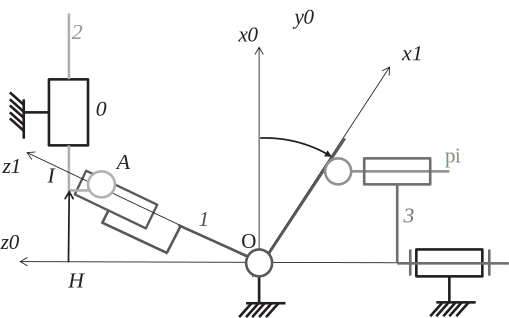
\includegraphics[width=.75\linewidth]{img/fig10}
\caption{\label{fig10}Modèle électrique du transducteur de couple en régime alternatif}
\end{center}
\end{minipage}\hfill
\begin{minipage}{0.45\linewidth}
\question{Exprimer les tensions $\underline{V_A}$ et $\underline{V_B}$ en fonction de $\underline{V_{12}}$ et des paramètres définis figure \ref{fig09}.}

\question{En déduire les expressions des paramètres $X_{var}$, $R_{tot}$ et $X_{tot}$ tels que :$\underline{V_S}=\dfrac{j\cdot X_{var}}{2\cdot (R_{tot}+j\cdot X_{tot})}\cdot \underline{V_{12}}$}

\question{Calculer la valeur de $R_{tot}$ ainsi que les valeurs extrémales de $X_{tot}$. Proposer alors une simplification de la grandeur $\left|\dfrac{\underline{V_S}}{\underline{V_{12}}}\right|$.}

\question{Indiquer la condition que doivent satisfaire les grandeurs $L_1$ et $\Delta L$ afin de pouvoir considérer le transducteur linéaire ($\underline{V_S}$ proportionnel à $\Delta L$).}
\end{minipage}
\end{figure}

\newpage

\subsection{Consommation énergétique du transducteur}

\paragraph{Objectif} Dimensionner les résistances $R_2$.

\textit{Rappel : le transducteur est étudié sur la base du modèle donné figure \ref{fig10}, les valeurs numériques relatives à ce modèle sont données figure \ref{fig09}.}

\paragraph{Exigence de consommation} Afin de respecter l'exigence 330 (figure \ref{fig06}), la puissance consommée par le transducteur ne doit pas dépasser 0.5 W.

\paragraph{Hypothèse supplémentaire} L'étude de la consommation énergétique du transducteur est menée en supposant $\Delta L = 0 H$.

\question{Montrer que la valeur du courant efficace $I_1=\dfrac{A}{\sqrt{R_1^2+(L_1\cdot \omega)^2}}$. Calculer sa valeur numérique. On rappelle que $V_{12}=2\cdot A$.}

\question{Exprimer la puissance $P_{trans}$ absorbée par le transducteur en fonction de $R_1$, $R_2$ et $A$.}

\question{Déduire des questions précédentes la valeur minimale de $R_2$ qui permet de limiter la puissance
$P_{trans}$ absorbée par le transducteur à $0.5W$.}

\section{Modélisation de l'association \{ onduleur + machine synchrone \}}

\paragraph{Objectif} Modéliser le fonctionnement de l'association \{ Machine synchrone à fcem trapézoïdales + onduleur \}.

Le groupe d'assistance est animé par une machine synchrone triphasée dont les forces contre-électromotrices
présentent une évolution temporelle trapézoïdale (figure \ref{fig11}).

\begin{figure}[ht!]
\begin{center}
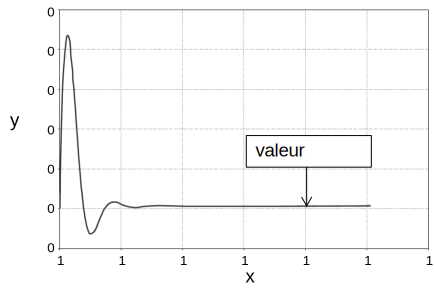
\includegraphics[width=.5\linewidth]{img/fig11}
\caption{\label{fig11}Forces électromotrices induites lors de la mise en rotation de la machine}
\end{center}
\end{figure}

Du fait de son comportement analogue à une machine à courant continu, l'association \{ machine à fcem trapézoïdales + onduleur \} porte la désignation
commerciale de \og machine à courant continu sans balais \fg (de l'anglais BLDC pour \og BrushLess Direct Courant motor \fg). Cette partie vise à modéliser le fonctionnement de cette association machine - modulateur.

Les grandeurs et notations utiles dans la suite de cette partie sont définies dans le tableau \ref{fig11} ainsi que sur les figures \ref{fig12} et \ref{fig13}. La figure \ref{fig13} détaille l'architecture de l'association onduleur + machine. L'onduleur est piloté de telle sorte que les courants $i_1$, $i_2$ et $i_3$ absorbés par chaque phase suivent le profil idéal défini figure \ref{fig12}.


\subsection{Acquisition du courant}

L'asservissement du courant absorbé par la machine est réalisé en appliquant une commande de type MLI
(modulation de largeur d'impulsion) sur les transistors. Les transistors pilotés évoluent en fonction de la phase électrique $\theta_e$. La résistance $R_s$ (figure \ref{fig13}) est un shunt de $3m\Omega$ utilisé pour l'acquisition du courant absorbé par la machine.

\begin{figure}[ht!]
\begin{center}
\includegraphics[width=.65\linewidth]{img/fig12}
\caption{\label{fig12}FCEM et courants idéaux dans chaque phase de la machine}
\end{center}
\end{figure}

\newpage

\begin{figure}[ht!]
\begin{center}
\includegraphics[width=.95\linewidth]{img/fig13}
\caption{\label{fig13}Machine synchrone à FEM trapézoïdale et modulateur associé}
\end{center}
\end{figure}

\paragraph{Séquence de commande des transistors} On s'intéresse au cas où $\theta_e$ est compris entre $30$ et $90\degree$. Au cours de cette phase, l'onduleur est piloté de la manière suivante :
\begin{itemize}
 \item les transistors $T_{3b}$ et $T_{3h}$ sont constamment bloqués (ouverts),
 \item le transistor $T_{2b}$ est constamment saturé (fermés),
 \item le transistor $T_{1h}$ est piloté de manière périodique. En notant $T$ la période de découpage et $\alpha$ le rapport cyclique de découpage, ce transistor est piloté de la manière suivante :
 \begin{itemize}
  \item $T_{1h}$ est saturé pour $t\in\left[0,\alpha\cdot T\right[$,
  \item $T_{1h}$ est bloqué pour $t\in\left[\alpha\cdot T,T\right[$.
 \end{itemize}
\end{itemize}

La période de découpage $T$ est choisie beaucoup plus petite que la période des FCEM.

\question{Sur le document réponse, surligner la maille dans laquelle circule un courant au cours de
chacun des deux temps de la période de découpage.}

\question{Tracer alors l'évolution temporelle de la tension aux bornes du shunt $R_s$ au cours
d'une période de découpage.}

\newpage

\section{Asservissement du couple délivré par le groupe d’assistance}

\begin{figure}[ht!]
\begin{minipage}{0.6\linewidth}
L’architecture du groupe d’assistance dont est pourvu le vélo est présentée figure \ref{fig16}. Ce groupe d’assistance ajoute au couple $C_{pc}$ appliqué par le cycliste sur le pédalier un couple $C_{pm}$ délivré par la motorisation. Ce système est asservi de telle sorte que le couple $C_{pm}$ appliqué par la motorisation est proportionnel au couple $C_{pc}$ fourni par le cycliste : $C_{pm}=K_{as}\cdot C_{pc}$ (le couple $C_{pm}$ sature à $90 N\cdot m$). Le cycliste peut faire varier le niveau d’assistance entre $0$ (groupe d’assistance désactivé) et $4$ (assistance maximale). Chaque niveau d’assistance correspond à une valeur du coefficient d’assistance $K_{as}$ (figure \ref{fig15}).
\end{minipage}\hfill
\begin{minipage}{0.35\linewidth}
\begin{center}
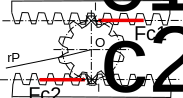
\includegraphics[width=.95\linewidth]{img/fig14}
\caption{\label{fig14}Évolution du coefficient d’assistance $K_{as}$ en fonction du niveau d’assistance}
\end{center}
\end{minipage}
\end{figure}

\paragraph{Cahier des charges de l’asservissement en couple} Les spécifications relatives à l’asservissement du couple appliqué par le groupe d’assistance au niveau de l’axe du pédalier sont données figure \ref{fig14}.

\begin{figure}[ht!]
\begin{center}
\includegraphics[width=.95\linewidth]{img/fig15}
\caption{\label{fig15}Extrait du cahier des charges relatif au contrôle du couple d’assistance}
\end{center}
\end{figure}

\newpage

\subsection{Modélisation de l’asservissement du couple $C_{pm}$}

L’asservissement du couple délivré par le groupe d’assistance est modélisé sous la forme du schéma-bloc
donné figure \ref{fig17}.

\paragraph{Notations et hypothèses}
\begin{itemize}
 \item $p$ désigne la variable de Laplace, la transformée de Laplace d’une fonction du temps $f(t)$ est notée $F(p)$,
 \item Les conditions de Heaviside sont supposées satisfaites.
 \item Les grandeurs introduites sur le schéma de la figure \ref{fig17} sont recensées dans le tableau \ref{tab01}.
\end{itemize}

\begin{figure}[ht!]
\begin{center}
\includegraphics[width=.9\linewidth]{img/fig16}
\caption{\label{fig16}Schéma d’architecture du groupe d’assistance}
\end{center}
\end{figure}

\begin{figure}[ht!]
\begin{center}
\includegraphics[width=.9\linewidth]{img/fig17}
\caption{\label{fig17}Schéma-bloc de l’asservissement du couple appliqué par le groupe d’assistance sur l’axe du pédalier}
\end{center}
\end{figure}

\newpage

\begin{table}[ht!]
\begin{tabular}{|p{0.7\linewidth}|p{0.1\linewidth}|p{0.2\linewidth}|}
\hline
\textbf{Grandeur} & \textbf{Symbole} & \textbf{Valeur} \\
\hline
Coefficient d’assistance (sans unité) & $K_{as}$ & \\
Fonction de transfert du correcteur & $C(p)$ & \\
\hline
Rapport de transmission du réducteur du groupe d’assistance & $K_r$ & 1/50 \\
Moment d’inertie de tout l’ensemble en mouvement ramené sur l’axe du pédalier & $J_{eq}$ & \\
Rapport de transmission du pédalier à la roue & $K_t$ & 42/12 \\
Rayon de la roue arrière & $R_1$ & 0.34m \\
Couple appliqué par le cycliste sur le pédalier & $C_{pc}(p)$ & \\
Couple appliqué par la motorisation sur le pédalier & $C_{pm}(p)$ & \\
Couple résistant ramené sur l’axe du pédalier & $C_{pr}(p)$ & \\
Vitesse de rotation du pédalier & $\Omega_{ped}(p)$ & \\ 
Vitesse de déplacement du vélo & $V_v(p)$ & \\
Masse de l’ensemble en mouvement & $m_T$ & 250kg\\
\hline
Constante de couplage & $K_m$ & $4\cdot 10^{-2}N\cdot m\cdot A^{-1}=4\cdot 10^{-2}V\cdot s\cdot rad^{-1}$\\
Résistance d’induit & $R_m$ & $0.1\Omega$ \\
Inductance d’induit & $L_m$ & $7\cdot 10^{-4}H$ \\
Force contre-électromotrice & $E(p)$ & \\
Tension d’induit & $U_m(p)$ &\\
\hline
\end{tabular}
\caption{\label{tab01}Grandeurs intervenant dans le schéma-bloc de la figure \ref{fig17}}
\end{table}

\paragraph{Énergies cinétiques et inertie équivalente} Au cours de son mouvement, le vélo accumule de l’énergie
cinétique :
\begin{itemize}
 \item de par son mouvement de translation par rapport au sol,
 \item du fait des rotations par rapport à son cadre de certains éléments composent le vélo (roues, rotor du
moteur, partie mobiles du réducteur, pédalier).
\end{itemize}

On admet que l’énergie cinétique accumulée par le mouvement de translation du vélo par rapport au sol est très
grande devant l’énergie cinétique accumulée par les mouvements de rotation.

\question{Déterminer la valeur du moment d’inertie équivalent $J_{eq}=m_T\cdot (R_1\cdot K_t)^2$ de l’ensemble du vélo ramené sur l’axe du pédalier.}

\newpage

\subsection{Simplification du modèle}

Le schéma-blocs donné figure \ref{fig17} peut se mettre sous la forme du schéma simplifié donné figure \ref{fig18}.

\begin{figure}[ht!]
\begin{center}
\includegraphics[width=.95\linewidth]{img/fig18}
\caption{\label{fig18}Schéma-bloc simplifié de l’asservissement du couple d’assistance}
\end{center}
\end{figure}

\question{À partir du schéma-bloc donné figure \ref{fig17}, déterminer la dimension de $C(p)$. Justifier alors
que les grandeurs $G_c$ et $G_{ped}$ sont homogènes.}

\question{Déterminer la fonction de transfert
$$H_G(p)=\dfrac{C_{pm}(p)}{\Delta G(p)}$$ en fonction de $C(p)$, $R_m$ et $L_m$.}

\question{Déterminer l’expression de $\Delta G(p)$ en fonction de $C_{pc}(p)$, $C_{pm}(p)$ et $C_{pr}(p)$ et des constantes du système.}

\subsection{Correction proportionnelle (P)}

\paragraph{Objectif} Évaluer le respect des exigences dans le cas d’une correction proportionnelle.

~\

On opte dans un premier temps pour une correction proportionnelle : $C(p)=K_c$.

\question{En supposant $C_{pr}=0$, déterminer l’expression de la fonction de transfert :
$$H_{as}(p)=\left.\dfrac{C_{pm}(p)}{C_{pc}(p)}\right|_{C_{pr}=0}$$

en fonction des grandeurs constantes définies dans le tableau \ref{tab01}.}

\question{Montrer alors que la correction proportionnelle ne permet pas de satisfaire l’exigence 420
portant sur l’erreur statique.}

\subsection{Correction proportionnelle intégrale (PI)}

\paragraph{Objectif} Dimensionner un correcteur proportionnel intégral permettant de satisfaire le cahier des charges.

~\

On évalue désormais le comportement de l’asservissement du couple d’assistance dans le cas d’une correction
proportionnelle-intégrale :

\begin{center}
$C(p)=K_c\dfrac{1+T_i\cdot p}{T_i\cdot p}$
\end{center}

Avec ce correcteur, la fonction de transfert $H_{as}(p)$ devient :
$$H_{as}(p)=\dfrac{K_{as}\cdot(K_r)^2\cdot J_{eq}\cdot K_c - (K_m)^2\cdot T_i + K_{as}\cdot (K_r)^2\cdot J_{eq} \cdot K_c\cdot T_i\cdot p}{Kc\cdot (K_r)^2\cdot J_{eq}+(K_m)^2\cdot T_i+(K_r)^2\cdot J_{eq}\cdot T_i\cdot \left[R_m+K_c\right]\cdot p+ (K_r)^2\cdot J_{eq}\cdot L_m\cdot T_i\cdot p^2}$$

\paragraph{Exigence de précision} Le respect de l’exigence 420 impose :
$$\dfrac{K_c}{T_i}\geq \dfrac{100+95\cdot K_{as}}{5\cdot K_{as}}\cdot\dfrac{(Km)^2}{K_r\cdot J_{eq}}$$
soit:$\dfrac{K_c}{T_i}\geq 12.3\cdot 10^{-3}V\cdot A^{-1}\cdot s^{-1}$ pour $K_{as}=0.5$ (cas le plus sévère).

\paragraph{Exigence de bande passante} Afin de respecter l’exigence 440 portant sur la bande passante de l’asservissement, on impose $\omega_0=252rad\cdot s^{-1}$.

\question{Exprimer le dénominateur de $H_{as}$ sous forme canonique et en déduire l’expression de sa pulsation propre $\omega_0$.}

\question{Déterminer la valeur du rapport $\dfrac{K_c}{T_i}$ qui permet d’obtenir $\omega_0=252rad\cdot s^{-1}$.}

\paragraph{Exigence portant sur les dépassements} Le concepteur a choisi de régler le coefficient d’amortissement $z$ à $1$ ce qui conduit aux valeurs suivantes : $K_c \approx 0.253 V\cdot A^{-1}\ et\  T_i\approx 5.69\cdot 10^{-3} s$.

\paragraph{Simulation} Le fonctionnement de l’asservissement du couple d’assistance est simulé pour $K_{as}=0.5$ avec les valeurs de $K_c$ et $T_i$ déterminées précédemment. De cette simulation sont extraits :
\begin{itemize}
 \item l’évolution du couple $C_{pm}$ en réponse à un échelon de couple $C_{pc}$ (figure \ref{fig19}),
 \item le diagramme de Bode du rapport $\dfrac{C_{pm}}{C_{pc}}$ (figure \ref{fig20}).
\end{itemize}

\question{Au regard du diagramme de Bode de la figure \ref{fig20}, proposer une forme simplifiée pour la
fonction de transfert $H_{as}$.}

\question{À partir des figures \ref{fig19} et \ref{fig20}, conclure quant au respect des exigences 420 et 430 du diagramme des exigences de la figure \ref{fig15}.}

\newpage

\begin{figure}[ht!]
\begin{center}
\includegraphics[width=.65\linewidth]{img/fig19}
\caption{\label{fig19}Évolution du couple d’assistance $C_{pm}$ pour $K_{as}=0.5$ en réponse à un échelon d’amplitude $80N\cdot m$ sur $C_{pc}$}
\end{center}
\end{figure}

\begin{figure}[ht!]
\begin{center}
\includegraphics[width=.8\linewidth]{img/fig20}
\caption{\label{fig20}Diagramme de Bode de la fonction de transfert $H_{as}(p)$ pour $K_{as}=0.5$}
\end{center}
\end{figure}

\finsujet

\debutcor

%1
\reponse{4}{}{
On isole le vélo, et on calcule le théorème du moment statique au point $G_v$ sur $\vec{z}$:
$$m_I\cdot x_G-m_J\cdot (L-x_G)=0\ donc\ x_G=\dfrac{m_J}{m_I+m_J}\cdot L$$

$$x_G=\dfrac{m_J}{m_I+m_J}\cdot L=\dfrac{24}{24+26}\cdot 2050=24\cdot 41=984mm$$
}

%2
\reponse{5}{}{
De même:
$(m_B+m_V)\cdot IG_T=m_B\cdot IG_B+m_V\cdot IG_V$ donc $(m_B+m_V)\cdot x_T=m_B\cdot	x_B+m_V\cdot x_V$, donc $x_T=\dfrac{m_B\cdot x_B+m_V\cdot x_G}{m_B+m_V}$

$x_T=\dfrac{100\cdot 1250+50\cdot 984}{100+50}=\dfrac{2500+984}{3}=833+328=1161mm$.
}

%3
\reponse{0}{\begin{center}
	\includegraphics[width=0.8\linewidth]{img/dr03.png}
\end{center}}{\begin{center}
   \def\svgwidth{0.8\linewidth}
   \input{img/dr03_cor.pdf_tex}
\end{center}}

%4
\reponse{0}{\begin{center}
	\includegraphics[width=0.8\linewidth]{img/dr04.png}
\end{center}}{\begin{center}
   \def\svgwidth{0.8\linewidth}
   \input{img/dr04_cor.pdf_tex}
\end{center}}

%5
\reponse{4}{}{
$\overrightarrow{IK}+\overrightarrow{KA}+\overrightarrow{AB}+\overrightarrow{BI}=\overrightarrow{0}$

$-\mu(t)\cdot\vec{x}+a\cdot\vec{x_b}-b\cdot\vec{x_c}+e\cdot\vec{y_c}-R_B\cdot\vec{y}=0$

en projetant sur $\vec{y}$, on obtient: $a\cdot sin\alpha=b\cdot sin\beta-e\cdot cos\beta+R_B$.
}

%6
\reponse{4}{}{$cos\beta=1$ et $sin\beta=0$, donc 

$a\cdot sin\alpha=R_B-e$

$sin\alpha=\dfrac{R_B-e}{a}=\dfrac{340-70}{290}=\dfrac{27}{29}\approx 0.9$

Ainsi, on retrouve graphiquement sur la figure \ref{fig04a} : $\alpha=63\degree$ ou $\alpha=180-63=117\degree$}

%7
\reponse{4}{}{On trouve $\beta_{max}=1.1\degree$, donc on peut valider l'hypothèse de $\beta$ petit et que le cadre est supposé horizontal lors du bequillage.}

%8
\reponse{3}{}{$\left\{T_{0\rightarrow 4}\right\}=\left\{
\begin{array}{c}X_{04}\cdot\vec{x}+Y_{04}\cdot\vec{y}\\ \vec{0}
\end{array}\right\}_K$}

%9
\reponse{3}{}{$\left\{T_{0\rightarrow 1}\right\}=\left\{
\begin{array}{c}X_{01}\cdot\vec{x}+Y_{01}\cdot\vec{y}\\ \vec{0}
\end{array}\right\}_I$}

%10
\reponse{3}{}{$\left\{T_{P\rightarrow \sum}\right\}=\left\{
\begin{array}{c}-m_T\cdot g\cdot\vec{y}\\ \vec{0}
\end{array}\right\}_{G_T}$}

%11
\reponse{11}{}{$\left\{T_{0\rightarrow 4}\right\}=\left\{
\begin{array}{c}X_{04}\cdot\vec{x}+Y_{04}\cdot\vec{y}\\ \vec{0}
\end{array}\right\}_K=\left\{
\begin{array}{c}X_{04}\cdot\vec{x}+Y_{04}\cdot\vec{y}\\-\mu\cdot Y_{04}\cdot\vec{z}
\end{array}\right\}_I$

$\left\{T_{0\rightarrow 1}\right\}=\left\{
\begin{array}{c}X_{01}\cdot\vec{x}+Y_{01}\cdot\vec{y}\\ \vec{0}
\end{array}\right\}_I$

$\left\{T_{P\rightarrow \sum}\right\}=\left\{
\begin{array}{c}-m_T\cdot g\cdot\vec{y}\\ \vec{0}
\end{array}\right\}_{G_T}=\left\{
\begin{array}{c}-m_T\cdot g\cdot\vec{y}\\(\mu-k\cdot\cos\beta+q\cdot\sin\beta)\cdot m_T\cdot g\cdot\vec{z}
\end{array}\right\}_I$

$\left\{T_{cycliste\rightarrow 4}\right\}=\left\{
\begin{array}{c}-F_c\cdot\vec{x}\\ \vec{0}
\end{array}\right\}_{M}=\left\{
\begin{array}{c}-F_c\cdot\vec{x}\\(a-d\cdot\sin\beta+y_M\cdot\cos\beta)\cdot F_c\cdot \vec{z}
\end{array}\right\}_I$

Donc: $-\mu\cdot Y_{04}+(\mu-k\cdot\cos\beta+q\cdot\sin\beta)\cdot m_T\cdot g+(a-d\cdot\sin\beta+y_M\cdot\cos\beta)\cdot F_c=0$

Donc, $F_c=\dfrac{\mu\cdot Y_{04}-(\mu-k\cdot\cos\beta+q\cdot\sin\beta)\cdot m_T\cdot g}{(a-d\cdot\sin\beta+y_M\cdot\cos\beta)}$
}

%12
\reponse{4}{}{$cos\beta=1$ et $sin\beta=0$, donc 

$F_c\approx\dfrac{\mu\cdot Y_{04}-(\mu-k)\cdot m_T\cdot g}{a+y_M}$

L'action est alors maximale si $y_M$ est minimale, soit $y_M=900mm$.}

%13
\reponse{4}{}{D'après les résultats de l'isolement:

$\left\{\begin{array}{l}
X_{01}+X_{04}-F_C=0\\
Y_{01}+Y_{04}-m_T\cdot g=0\\
\end{array}\right.$}

%14
\reponse{3}{}{Il y a 3 équations liées à l'isolement + 1 liée au glissement en I, soit 4 équations et 5 inconnues ($X_{04}$, $Y_{04}$, $X_{01}$, $Y_{01}$ et $F_C$), il n'est pas possible de résoudre.}

%15
\reponse{3}{}{On isole la béquille (4) et on applique le théorème du moment statique en A:
$a\cdot X_{04}+0=0$, donc $X_{04}=0$.
}

%16
\reponse{3}{}{Une femme ne peut pas exercer un effort de plus de 70N 30 fois par jour, cela ne permet donc pas d'effectuer des livraisons.}

%17
\reponse{2}{}{Si A est nulle, alors $v_s=0$ et les sources ne délivrent aucune tension.}

%18
\reponse{4}{}{$\underline{V_A}=\dfrac{R_1+j\cdot(L_1+\Delta L)\cdot\omega}{R_1+j\cdot L_1\cdot\omega+R_1+j\cdot(L_1+\Delta L)\cdot\omega}\cdot\underline{V_{12}}=\dfrac{1}{2}\cdot\dfrac{R_1+j\cdot(L_1+\Delta L)\cdot\omega}{R_1+j\cdot \left(L_1+\dfrac{\Delta L}{2}\right)\cdot\omega}\cdot\underline{V_{12}}$

De même, $\underline{V_B}=\dfrac{R_2}{R_2+R_2}\cdot\underline{V_{12}}=\dfrac{1}{2}\cdot\underline{V_{12}}$}

%19
\reponse{4}{}{D'après la loi des mailles : $\underline{V_A}=\underline{V_S}+\underline{V_B}$, donc 

$\underline{V_S}=\underline{V_A}-\underline{V_B}=\dfrac{1}{2}\cdot\dfrac{j\cdot\dfrac{\Delta L}{2}\cdot\omega}{R_1+j\cdot \left(L_1+\dfrac{\Delta L}{2}\right)\cdot\omega}\cdot\underline{V_{12}}$

Donc, $R_{tot}=R_1$, $X_{var}=\dfrac{\Delta L}{2}\cdot\omega$ et $X_{tot}=\left(L_1+\dfrac{\Delta L}{2}\right)\cdot\omega$}

%20
\reponse{4}{}{$R_{tot}=5\Omega$

$X_{tot\ max}=L_1\cdot\omega=5\cdot 10^{-3}\cdot 2\cdot \pi\cdot 20\cdot 10^3=200\cdot\pi=628\Omega$

$X_{tot\ min}=\left(L_1-\dfrac{\Delta L_{Max}}{2}\right)\cdot\omega=4.5\cdot 2\cdot \pi\cdot 20=180\cdot \pi=628-62,8=565,2\Omega$

On voit que $R_{tot}$ est négligeable devant $X_{tot}$, donc $\dfrac{\underline{V_S}}{\underline{V_{12}}}=\dfrac{X_{var}}{2\cdot X_{tot}}=\dfrac{\Delta L}{4\cdot \left(L_1+\dfrac{\Delta L}{2}\right)}$.}

%21
\reponse{4}{}{
$\underline{V_S}$ est proportionnel à $\Delta L$ si $L_1+\dfrac{\Delta L}{2}$ est constant, donc si $L_1>>\dfrac{\Delta L}{2}$, dans ce cas, 

$\dfrac{\underline{V_S}}{\underline{V_{12}}}=\dfrac{\Delta L}{4\cdot L_1}$.}

%22
\reponse{2}{}{
$I_1=\dfrac{V_{12}}{2\cdot|\underline{Z_1}|}=\dfrac{A}{\sqrt{R_1^2+(L_1\cdot\omega)^2}}=\dfrac{8}{\sqrt{5^2+(5\cdot 10^{-3}\cdot 2\cdot\pi\cdot 20\cdot10^3)^2}}=\dfrac{8}{\sqrt{5^2+(200\cdot\pi)^2}}\approx\dfrac{8}{200\cdot\pi}\approx\dfrac{12}{1000}\approx 12mA$}

%23
\reponse{4}{}{La puissance est absorbée par les résistances, donc $P_{trans}=2\cdot P_{R_1}+2\cdot P_{R_2}=2\cdot R_1\cdot I_1^2+2\cdot \dfrac{V_{12}^2}{4\cdot R_2}=\dfrac{2\cdot R_1\cdot A^2}{R_1^2+(L_1\cdot\omega)^2}+\dfrac{2\cdot A^2}{R_2}$}

%24
\reponse{4}{}{

$\dfrac{2\cdot R_1\cdot A^2}{R_1^2+(L_1\cdot\omega)^2}+\dfrac{2\cdot A^2}{R_2}\leq\dfrac{1}{2}$

$\dfrac{2\cdot A^2}{R_2}\leq\dfrac{1}{2}-\dfrac{2\cdot R_1\cdot A^2}{R_1^2+(L_1\cdot\omega)^2}$

$\dfrac{2\cdot A^2}{R_2}\leq\dfrac{R_1^2+(L_1\cdot\omega)^2-4\cdot R_1\cdot A^2}{2\cdot\left(R_1^2+(L_1\cdot\omega)^2\right)}$

$R_{2\ min}=\dfrac{4\cdot A^2\cdot\left(R_1^2+(L_1\cdot\omega)^2\right)}{R_1^2+(L_1\cdot\omega)^2-4\cdot R_1\cdot A^2}$

$R_{2\ min}=\dfrac{4\cdot 8^2\cdot\left(5^2+(5\cdot 2\cdot \pi\cdot 20)^2\right)}{5^2+(5\cdot 2\cdot \pi\cdot 20)^2-4\cdot 5\cdot 8^2}$

$R_{2\ min}=\dfrac{256\cdot\left(25+(200\cdot \pi)^2\right)}{25+(200\cdot \pi)^2-1280}\approx 256\Omega$}

%25
\reponse{0}{\begin{center}
	\includegraphics[width=0.8\linewidth]{img/dr25.png}
\end{center}}{\begin{center}
   \def\svgwidth{0.8\linewidth}
   \input{img/dr25_cor.pdf_tex}
\end{center}}

%26
\reponse{4}{}{Pour $t\in[0,\alpha\cdot T[ \rightarrow i_S=i_{10}$

Pour $t\in[\alpha\cdot T,T[ \rightarrow i_S=0$

\begin{center}
   \def\svgwidth{0.8\linewidth}
   \input{img/dr26_cor.pdf_tex}
\end{center}}

%27
\reponse{2}{}{
$J_{eq}=m_T\cdot(R_1\cdot K_t)^2=250\cdot \left(0.34\cdot \dfrac{42}{12}\right)^2=250\cdot (0.17\cdot 7)^2=250\cdot 0.0289\cdot 49=250\cdot 1.5=375kg\cdot m^2$
}

%28
\reponse{2}{}{

L'entrée de $C(p)$ est un courant, la sortie une tension, alors $C(p)$ est homogène à des $\Omega$.

\begin{itemize}
 \item $G_c(p)$ est en $V\cdot A^{-1}\cdot N\cdot m$,
 \item $G_{ped}(p)$ est en $(N\cdot m\cdot A^{-1})(V\cdot s\cdot rad^{-1})(rad\cdot s^{-1})$, soit des $N\cdot m\cdot A^{-1}\cdot V$ comme $G_c(p)$ .
\end{itemize}}

%29
\reponse{2}{}{
$H_G(p)=\dfrac{C_{pm}(p)}{\Delta G(p)}=\dfrac{\dfrac{1}{R_m+L_m\cdot p}}{1+\dfrac{C(p)}{R_m+L_m\cdot p}}$

$H_G(p)=\dfrac{1}{C(p)+R_m+L_m\cdot p}$
}

%30
\reponse{4}{}{
$\Delta G(p)=G_c(p)-G_{ped}(p)$

$G_c(p)=K_{as}\cdot C(p)\cdot C_{pc}(p)$

$G_{ped}(p)=\left(\dfrac{K_m}{K_r}\right)^2\cdot\dfrac{1}{J_{eq}\cdot p}\cdot C_{pt}(p)$

$C_{pt}(p)=C_{pc}(p)+C_{pm}(p)-C_{pr}(p)$

$\Delta G(p)=\left[K_{as}\cdot C(p)-\left(\dfrac{K_m}{K_r}\right)^2\cdot\dfrac{1}{J_{eq}\cdot p}\right]\cdot C_{pc}(p)-\left(\dfrac{K_m}{K_r}\right)^2\cdot\dfrac{1}{J_{eq}\cdot p}\left(C_{pm}(p)-C_{pr}(p)\right)$
}

%31
\reponse{4}{}{
$C_{pm}(p)=H_G(p)\cdot \Delta G(p)$ et $\Delta G(p)=K_{as}\cdot K_c\cdot C_{pc}(p)-\left(\dfrac{K_m}{K_r}\right)^2\cdot\dfrac{1}{J_{eq}\cdot p}\cdot\left(C_{pm}(p)+C_{pc}(p)\right)$

$C_{pm}(p)=H_G(p)\cdot \left[K_{as}\cdot K_c\cdot C_{pc}(p)-\left(\dfrac{K_m}{K_r}\right)^2\cdot\dfrac{1}{J_{eq}\cdot p}\cdot\left(C_{pm}(p)+C_{pc}(p)\right)\right]$

$C_{pm}(p)\left(1+\dfrac{1}{K_c+R_m+L_m\cdot p}\cdot\left(\dfrac{K_m}{K_r}\right)^2\cdot\dfrac{1}{J_{eq}\cdot p} \right)=\dfrac{1}{K_c+R_m+L_m\cdot p}\cdot\left(K_{as}\cdot K_c-\left(\dfrac{K_m}{K_r}\right)^2\cdot\dfrac{1}{J_{eq}\cdot p}\right)\cdot C_{pc}(p)$

$H_{as}(p)=\dfrac{\dfrac{1}{K_c+R_m+L_m\cdot p}\cdot\left(K_{as}\cdot K_c-\left(\dfrac{K_m}{K_r}\right)^2\cdot\dfrac{1}{J_{eq}\cdot p}\right)}{1+\dfrac{1}{K_c+R_m+L_m\cdot p}\cdot\left(\dfrac{K_m}{K_r}\right)^2\cdot\dfrac{1}{J_{eq}\cdot p}}$

$H_{as}(p)=\dfrac{K_{as}\cdot K_c-\left(\dfrac{K_m}{K_r}\right)^2\cdot\dfrac{1}{J_{eq}\cdot p}}{\left(K_c+R_m+L_m\cdot p\right)+\left(\dfrac{K_m}{K_r}\right)^2\cdot\dfrac{1}{J_{eq}\cdot p}}$

$H_{as}(p)=-\left(\dfrac{1-\dfrac{K_{as}\cdot K_c\cdot K_r^2\cdot J_{eq}}{K_m^2}\cdot p}{1+\dfrac{K_p^2}{K_m^2}\cdot J_{eq}\cdot\left(K_c+R_m\right)\cdot p+\dfrac{K_p^2}{K_m^2}\cdot L_m\cdot J_{eq}\cdot p^2}\right)$
}

%32
\reponse{4}{}{
Soit l'entrée $C_{pc}(p)=\dfrac{C_{p0}}{p}$

$\lim\limits_{t\rightarrow +\infty} C_{pm}(t)=\lim\limits_{p\rightarrow 0} p\cdot C_{pm}(p)=-C_{p0}$

$\lim\limits_{t\rightarrow +\infty} (K_{as}\cdot C_{p0}-C_{pm}(t))=(K_{as}+1)\cdot C_{p0}$

On a alors:\\
\begin{tabular}{|c|c|c|}
\hline
$K_{as}$&$0.05\cdot K_{as}$&$1+K_{as}$\\ 
\hline
0&0&1\\
\hline
0.5&0.025&1.5\\
\hline
1&0.05&2\\
\hline
2&0.1&3\\
\hline
4&0.2&5\\
\hline
\end{tabular}

$(1+K_{as})\cdot C_{p0}>0.05\cdot K_{as}\cdot C_{p0}$, donc l'exigence 420 n'est pas respectée.
}

%33
\reponse{3}{}{

Soit, $D(p)$ le dénominateur de $H_{as}(p)$.

$D(p)=Kc\cdot (K_r)^2\cdot J_{eq}+(K_m)^2\cdot T_i+(K_r)^2\cdot J_{eq}\cdot T_i\cdot \left[R_m+K_c\right]\cdot p+ (K_r)^2\cdot J_{eq}\cdot L_m\cdot T_i\cdot p^2$

$D(p)=\left(Kc\cdot K_r^2\cdot J_{eq}+K_m^2\cdot T_i\right)\cdot\left(1+\dfrac{K_r^2\cdot J_{eq}\cdot T_i\cdot \left[R_m+K_c\right]}{Kc\cdot K_r^2\cdot J_{eq}+K_m^2\cdot T_i}\cdot p+\dfrac{K_r^2\cdot J_{eq}\cdot T_i\cdot L_m}{Kc\cdot K_r^2\cdot J_{eq}+K_m^2\cdot T_i}\cdot p^2\right)$

Donc, $\omega_0=\sqrt{\dfrac{Kc\cdot K_r^2\cdot J_{eq}+K_m^2\cdot T_i}{K_r^2\cdot J_{eq}\cdot T_i\cdot L_m}}$.
}

%34
\reponse{3}{}{
$\omega_0^2=\dfrac{Kc\cdot K_r^2\cdot J_{eq}+K_m^2\cdot T_i}{K_r^2\cdot J_{eq}\cdot T_i\cdot L_m}\Leftrightarrow
\omega_0^2=\dfrac{Kc}{T_i\cdot L_m}+\dfrac{K_m^2}{K_r^2\cdot J_{eq}\cdot L_m} \Leftrightarrow
\dfrac{Kc}{T_i}=L_m\cdot\left(\omega_0^2-\dfrac{K_m^2}{K_r^2\cdot J_{eq}\cdot L_m}\right) \Leftrightarrow
\dfrac{Kc}{T_i}=L_m\cdot\omega_0^2-\dfrac{K_m^2}{K_r^2\cdot J_{eq}} \Leftrightarrow
\dfrac{Kc}{T_i}=7\cdot 10^{-4}\cdot 252^2-\dfrac{(4\cdot 10^{-2})^2}{\left(\dfrac{1}{50}\right)^2\cdot 360} \Leftrightarrow
\dfrac{Kc}{T_i}=44-\dfrac{16\cdot 10^{-4}}{\dfrac{1}{250}\cdot 360} \Leftrightarrow
\dfrac{Kc}{T_i}\approx 44V\cdot A^{-1}\cdot s^{-1}$}

%35
\reponse{3}{}{
On peut reconnaître une fonction du 1er ordre $H_{as}(p)=\dfrac{K_{as}}{1+\tau_{as}\cdot p}$.

On lit:
\begin{itemize}
 \item $20\cdot\log(K_{as})=-6$, donc $K_{as}=0.5$,
 \item $\dfrac{1}{400}s\leq\tau_{as}\leq \dfrac{1}{300} s\Rightarrow 2.5ms\leq\tau_{as}\leq 3.3ms$.
\end{itemize}
}

%36
\reponse{3}{}{
L'erreur statique est $0.5\cdot 80-39,9829=0,0171N\cdot m<5\%\cdot 40$, donc 420 est respectée.

Le dépassement est de $\dfrac{40.6113-39.9829}{39.9829}=\dfrac{0.6284}{39.9829}\approx 0.015<5\%$, donc 430 est respectée.
}

\end{document}